\chapter{PhoG: Numerical methods}\label{appendix:phog_numerical_methods}

In this appendix we will briefly overview the numerical methods which are used in Chapter~\ref{chapter:phog}. The first two methods, direct integration in Sec.~\ref{appendix:direct_integration}, and quantum Monte Carlo in Sec.~\ref{appendix:monte_carlo}, are standard methods for handling the Lindblad master equation. %There is much written about them elsewhere \cite{Plenio1998, Daley2014} and so will discuss them only briefly. 
The final two methods, mean-field and linearization, Secs.~\ref{appendix:single_mode_mean_field},~\ref{appendix:single_mode_linear},~\ref{appendix:mean_field},~\ref{appendix:multi_mode_linear}, are discussed at length in the main body of the Thesis, Sec.~\ref{sec:phog_multi_mode}, and so we will just reproduce the final systems of equations in this Appendix. %Sample Python code which implements the direct integration method and the quantum monte carlo method for this Thesis is available at Ref.~\cite{deposited_code}.

\section{Direct integration}\label{appendix:direct_integration}

The dynamics of a quantum system coupled to a reservoir is governed by the Lindblad equation
\begin{equation}\label{eqn:appendix_lindblad}
\ddt \rho = - i \left[ \hat{H}, \rho \right] + \sum_n \left(\hat{C}_n \rho \hat{C}_n^\dagger - \frac{1}{2} \hat{C}_n^\dagger \hat{C}_n \rho - \frac{1}{2} \rho \hat{C}_n^\dagger \hat{C}_n \right),
\end{equation}
where $\hat{H}$ acts only on $\rho$ and $\hat{C}_n$ are the collapse operators governing decay into the reservoir. Here we take $\hat{C}_n = \sqrt{\gamma_n} \hat{A}_n$ where $\hat{A}_n$ is an operator acting on $\rho$. This is the operator through which $\rho$ couples to the reservoir in the original system-reservoir Schr{\"o}dinger equation. The derivation of this Lindblad equation including requisite approximations is discussed extensively in many canonical texts such as Refs.~\cite{Breuer2002, Carmichael1999}. 

There are many routes which one can take to solve Eq.~\ref{eqn:appendix_lindblad}. One such approach is to interpret $\rho$, $\hat{H}$ and $\hat{C}_n$ as matrices. Let our underlying Hilbert-space be denoted $\mathcal{H}$ and have dimension $\dims$. Then $\rho$, $\hat{H}$ and $\hat{C}_n$ each have dimension $\dims^2$ and may be interpreted as a matrices in $M_{\dims \times \dims}\left(\mathbb{C}\right)$. In this approach, the Lindblad equation~\ref{eqn:appendix_lindblad} can be interpreted as a coupled system of $\dims^2$ first-order ODEs, which can then be solved via an appropriate numerical method \cite{Corless2013}, the efficiency and power of which will depend strongly on the choices of $\hat{H}$, $\hat{C}_n$ and initial condition $\rho\left(0\right)$.

It should be noted that such an approach will only ever give an approximation to the true systems which we study in this Thesis. The key reason for this is that the quantum states we begin with are coherent states which take the form

\begin{equation}\label{eqn:appendix_coherent}
\ket{\alpha} = e^{-\frac{\left|\alpha\right|^2}{2}}\sum_{n=0}^\infty \frac{\alpha^n}{\sqrt{n!}}\ket{n}
\end{equation}
where $\ket{n}$ is the $n$-photon Fock state. %TODO: Ensure that Fock state is in the introduction
The sum in Eq.~\ref{eqn:appendix_coherent} runs from zero to infinity and so the required Hilbert space size is countably infinite. However, for any given $\alpha$, is is possible to find $N$ such that the state
\begin{equation}\label{eqn:appendix_coherent_state_truncated}
\ket{\psi} = e^{-\frac{\left|\alpha\right|^2}{2}}\sum_{n=0}^N \frac{\alpha^n}{\sqrt{n!}}\ket{n}
\end{equation} 
has both $\left| \ip{\psi} \right|^2 \approx 1$ and $\ip{\alpha}{\psi} \approx 1$. Thus, truncating the countable Hilbert space to a large but finite one should be possible. In this Thesis we use truncation values such that all states are appropriately normalized and that no ill effects are introduced from the truncation to a finite $\dims$. A good rule-of-thumb is to pick
\begin{equation}\label{eqn:rule_of_thumb}
\dims \ge \lceil 2 \alpha^2 \rceil
\end{equation}
which ensures that the coherent state Eq.~\ref{eqn:appendix_coherent_state_truncated} is correctly normalized and a good approximation of the full Eq.~\ref{eqn:appendix_coherent}. For all simulations $N$ was then increased until there was no change in the resulting dynamics.

In this Thesis we make use of open-source QuTiP package\footnote{QuTiP version $4.4.1$; Numpy version $1.16.4$; Scipy version $1.3.1$; Cython version $0.29.13$; Matplotlib version $3.1.0$; Python version $3.7.4$.} \cite{qutip2} in Python to perform such numerical solutions. The coherent state must be defined in QuTiP specifying the ``analytic" option to \code{qutip.coherent\_dm}, which ensures that $\dyad{\alpha}$ uses the expression Eq.~\ref{eqn:appendix_coherent_state_truncated}. The default option, ``operator,'' instead finds the eigenstate of annihilation operator $\hat{a}$. As $\dims \rightarrow \infty$ these two forms of coherent state become equivalent, but for small $\dims$ they can differ significantly. We have found that the analytic form gives much more accurate behaviour in the parameter ranges considered and requires smaller $\dims$ to give an accurate representation of the resulting dynamics.

Direct integration of the ODE system is performed using the \code{qutip.mesolve} command, which itself calls \code{scipy.integrate.ode}. On a standard home-use laptop\footnote{Intel(R) Core(TM) i$5-3230$M CPU $@ 2.60$~GHz; $8.00$~GB RAM.} a single-mode system with $\dims = 35$, initial $\rho\left(0\right)$ a coherent state with $\alpha = 3.0$, decay rate $\gamma = 1.0$, collapse operator $\hat{a}$ and free Hamiltonian $\hat{H} = \omega \hat{a}^\dagger \hat{a}$ with $\omega = 1.0$ can be solved in\footnote{Timed via iPython \code{\%timeit} magic command.} $41.7$~ms $\pm 11.7$~ms. Setting $\dims = 50$ takes $92.6 \pm 3$~ms, $\dims = 200$ takes $829$~ms $\pm 191$~ms.

However, using collapse operator $\ncl$ increases the computational power required, %and $\dims = 10$ takes $341$~ms $\pm 77.2$~ms, 
and $\dims = 35$ takes $11.3$~s $\pm 1.64$~s, and $\dims=100$ takes $110$~s. %Larger $\dims$ are intractable.
We see then that this approach is highly dependent on both the form of $\hat{H}, \hat{C}_n$ and the Hilbert-space size. Indeed, a Hilbert space size $\dims$ yields $\dims^2$ coupled ODEs\footnote{Including more modes in our model means the number of equations increases even faster. For two modes, living on Hilbert spaces $\mathcal{H}_A, \mathcal{H}_B$, the total system size is $\left| \mathcal{H}_A \otimes \mathcal{H}_B \right| = \left|\mathcal{H}_A\right| \times \left| \mathcal{H}_B\right|$.} to solve. We compare timings between direct integration and quantum Monte Carlo methods in Tab.~\ref{table:numerical_methods}.

%\MT{mention about scaling with number of modes}


\section{Quantum Monte Carlo}\label{appendix:monte_carlo}
We have seen that direct integration of Eq.~\ref{eqn:appendix_lindblad} requires a system of $\dims^2$ coupled ODEs to be simultaneously solved. This is possible in the limit of small $\dims$, but quickly becomes difficult as $\dims$ increases. An alternative approach does not solve a matrix differential equation, rather a vector one, and so instead scales as $\dims$.

%\MT{cite a bunch of stuff about non-Hermitian Hamiltonians}

We will outline the quantum Monte Carlo (QMC) approach and then discuss its implementation and use in this Thesis. The key principle of the QMC approach is to solve the Schr{\"o}dinger equation,
\begin{equation}\label{eqn:schrodinger}
i \ddt \ket{\psi} = \hat{H}\ket{\psi},
\end{equation}
instead of the Lindblad equation. The Schr{\"o}dinger equation is an equation for ket vector $\ket{\psi}$ rather than density matrix $\dyad{\psi}$, and so requires fewer computational resources. The Hamiltonian $\hat{H} = \hat{H}_{\text{eff}}$ should be chosen as
\begin{equation}
\hat{H}_{\text{eff}} = \hat{H}_{\text{sys}} + \hat{H}_{\text{non-Hermitian}}
\end{equation}
where $\hat{H}_{\text{sys}}$ is the system Hamiltonian, identical to the $\hat{H}$ used in the Lindblad equation~\ref{eqn:appendix_lindblad}, while 
\begin{equation}
\hat{H}_{\text{non-Hermitian}} = -\frac{i}{2} \sum_n \hat{C}_n^\dagger \hat{C}_n
\end{equation}
is a non-Hermitian Hamiltonian which causes dissipation to the state $\ket{\psi}$ via collapse operators $\hat{C}_n$. The non-Hermitian Hamiltonian does not conserve the norm of $\ket{\psi}$. QuTiP leverages this behaviour into the following algorithm which models a single trajectory of evolution of $\ket{\psi}$ \cite{Plenio1998, Dum1992, Dalibard1992, Daley2014}.

Choose a number $r \in \left(0, 1\right)$ uniformly at random. This number is related to the collapse probability of $\ket{\psi}$ caused by the $\hat{C}_n$. The Schr{\"o}dinger equation Eq.~\ref{eqn:schrodinger} is numerically integrated\footnote{QuTiP calls \code{scipy.integrate.ode}} and the norm $\ip{\psi\left(t\right)}$ is monitored.  

At time $\tau$ such that $\ip{\psi\left(\tau\right)} = r$, project $\ket{\psi\left(\tau\right)}$ onto $\hat{C}_n \ket{\psi\left(\tau\right)}$ and re-normalize. This is referred to as a ``jump''. So
\begin{equation}\label{eqn:appendix_jump}
\ket{\psi\left(\tau\right)} \rightarrow \frac{\hat{C}_n \ket{\psi\left(\tau\right)}}{\sqrt{\bra{\psi\left(\tau\right)}\hat{C}_n^\dagger \hat{C}_n \ket{\psi\left(\tau\right)}}}.
\end{equation}

\noindent Draw another $r \in \left(0, 1\right)$ and continue the evolution using the new $\ket{\psi}$ as the starting point. This process is repeated until the entire temporal range is covered. This gives us a single trajectory of the evolution of $\ket{\psi}$. 

The above procedure is repeated many times, and observables should be averaged\footnote{Simply using \code{numpy.mean} at each timestep} over many trajectories. It can be shown that this procedure implements the corresponding Lindblad master equation \cite{Plenio1998, Leonhardt2010} by noticing that the evolution from $\dyad{\psi\left(t\right)}$ to $\dyad{\psi\left(t + \Delta t\right)}$ is effectively a mixture over whether a jump occurred or not:
\begin{align}
\dyad{\psi}\left(t + \Delta t\right)  = \Delta P \dyad{\psi_{\text{Jump}}} + \left(1 - \Delta P\right) \dyad{\psi_{\text{No Jump}}}
\end{align}
The state $\ket{\psi_{\text{Jump}}}$ is given by Eq.~\ref{eqn:appendix_jump}, while $\ket{\psi_{\text{No Jump}}}$ is found by explicitly enacting the non-Hermitian effective Hamiltonian on $\ket{\psi}$ for $\Delta t$. By substituting in our expressions and allowing $\Delta t \rightarrow 0$, this reduces to a Lindblad equation of our original form. %TODO: make sure that I can do this for the viva.



Let us consider the performance of the QMC method and compare it to direct integration. QMC may be implemented by using \code{qutip.mcsolve} and specifying $\hat{H}_{\text{sys}}$, $\ket{\psi\left(0\right)}$, $\hat{C}_n$ and the operators $\hat{E}_n$ whose expectations should be measured. Let us solve an identical system to the one discussed in Eq.~\ref{appendix:direct_integration}: a single-mode system consisting of an initial coherent state with $\alpha = 3.0$, decay rate $\gamma = 8.0$ with collapse operator $\hat{a}$, and let us measure the photon-number expectation $\ev{\hat{a}^\dagger \hat{a}}$. 

For $\dims = 35$, the QMC method takes $12.40$~s to model $500$~trajectories. This performance is worse than for direct-integration, owing to the high overhead to average a large number of trajectories. Function \code{qutip.mcsolve} also naturally uses parallel-processing functionality\footnote{Provided by \code{multiprocessing.Pool}} which has high overhead. $\dims = 50$ takes $11.61$~s and $\dims = 200$ takes $19.08$~s.

We compare the speed of the direct integration and QMC approaches to solve Eq.~\ref{eqn:phog_single_mode_deriv} with $\gamma = 1.0$, varying initial coherent state amplitude and decay operator $\ncl$ in Tab.~\ref{table:numerical_methods}. All states were correctly normalized, which implies that the earlier condition Eq.~\ref{eqn:rule_of_thumb} is only a rule-of-thumb. We compare the QMC and direct integration methods for accuracy in Fig.~\ref{fig:appendix_numerical_methods_comparisons}.



\begin{table*}
	\captionsetup{width=0.8\linewidth}
	\centering \ra{1.75}
	\begin{tabular*}{0.8\textwidth}{@{\extracolsep{\stretch{1}}} cc c cc c}
	\multicolumn{2}{c}{\textbf{Run parameters}} && 
	\multicolumn{2}{c}{\textbf{Timings}} \\
	\hline 
	\head{$\dims$} & \head{$\alpha$} && \head{DI $[\si{s}]$} & \head{QMC $[\si{s}]$}
	\\
	\hline
	\phantom{0}35 & \phantom{0}3.0 && \phantom{0}0.048 & \phantom{0}\phantom{0}10.33 \\ 
	\phantom{0}50 & \phantom{0}5.0 && \phantom{0}0.145 & \phantom{0}\phantom{0}11.05 \\ 
	100 & \phantom{0}8.0 && \phantom{0}0.319 & \phantom{0}\phantom{0}14.84 \\  
	200 & 12.0 && \phantom{0}\phantom{0}4.04 & \phantom{0}\phantom{0}29.68 \\ 
	500 & 20.0 && 332.32 & \phantom{0}143.84 \\ 
	750 & 25.0 && - & \phantom{0}224.00 \\ 
	1500 & 37.0 && - & \phantom{0}753.05 \\ 
	1950 & 38.0 && - & 1361.72 \\
	\end{tabular*}
	\caption{\label{table:numerical_methods} Run-times to solve Eq.~\ref{eqn:phog_single_mode_deriv} with $\gamma_L = 10.0$, $\gamma_2 = 0.0005$, $\gncl = 0.002$, input coherent state amplitude $\alpha$ and $500$ QMC trajectories. Missing direct integration entries returned memory errors.}
\end{table*}
	


\begin{figure}[htp]
\captionsetup{width=0.8\linewidth}
\centering
\includegraphics[draft=false, width=0.7\linewidth]{phog/DI_QMC_comparison_gamma1=0}
\caption{\label{fig:appendix_numerical_methods_comparisons} Comparison of accuracy between direct integration and quantum monte carlo methods with varying number of monte carlo trajectories $n_{traj}$. Solving Eq.~\ref{eqn:phog_single_mode_deriv} with $\gamma_L = 10.0$, $\gamma_2 = 0.0005$, $\gamma_3 = 0.002$, $\dims = 500$, $\alpha = 20.0$. Dashed: direct integration. Solid: quantum monte carlo. For $n_{traj}$ small the behaviour is qualitatively similar to the full solution, but we must choose large $n_{traj}$ in order to make accurate quantitative predictions. For this thesis we take $n_{traj}=500$ unless otherwise stated.}
\end{figure}

\clearpage
\section{Mean-field single-mode model}\label{appendix:single_mode_mean_field}
Applying the mean-field approximation discussed in Sec.~\ref{sec:meanfield}to the single-mode PhoG model Eq.~\ref{eqn:phog_single_mode_deriv}, we arrive at the following equation for first-order expectation $\ev{s_-}$:

\begin{align}
&\ddt \ev{s_-} = - \frac{\gamma_1}{2} \ev{s_-} - i \varsigma_1 \ev{s_-} - i \varsigma_3 \ev{s_-} - 2 i \varsigma_1 \ev*{s_-^\dagger} \ev{s_-} \ev{s_-}  \notag \\
%
&- \gamma_2 \ev*{s_-^\dagger} \ev{s_-} \ev{s_-} - \gamma_3 \ev*{s_-^\dagger} \ev{s_-} \ev{s_-} - \frac{\gamma_3}{2} \ev*{s_-^\dagger} \ev*{s_-^\dagger} \ev{s_-} \ev{s_-} \ev{s_-}
\end{align}

\noindent with $\ev*{s_-^\dagger} = \ev{s_-}^*$. The system may be readily solved for $\ev{s_-}\left(t\right)$.

\section{Linearized single-mode model}\label{appendix:single_mode_linear}
By applying the linearization approximations derived in Sec.~\ref{sec:linearization} to the system of coupled ODEs derived from single-mode Lindblad equation~\ref{eqn:phog_single_mode_deriv} we arrive at the following closed system of ODEs:


\begin{align}%\label{eqn:expectations_linear_first}
%
%a
%
\partial_t\langle s_- \rangle &= c_1 \langle s_- \rangle + c_2 \left(\langle s_-^\dagger \rangle \langle s_-^2 \rangle + 2 \langle s_- \rangle \langle n_-\rangle - 2 \langle s_-^\dagger \rangle \langle s_- \rangle^2\right) \notag \\
%
&-\frac{\gamma_3}{2}\left(
6 \langle s_-^\dagger \rangle \langle n_- \rangle \langle s_-^2\rangle + 3 \langle s_- \rangle \langle s_-^{\dagger 2} \rangle \langle s_-^2 \rangle \right. \notag \\
%
&+ 6 \langle s_- \rangle \langle n_- \rangle^2 - 2 \langle s_-^{\dagger 2} \rangle \langle s_- \rangle^3 - 12 \langle n_- \rangle \langle s_-^\dagger \rangle \langle s_- \rangle^2 \notag \\
%
&\left. - 6 \langle s_-^2 \rangle \langle s_-^\dagger \rangle^2 \langle s_- \rangle + 6 \langle s_-^\dagger \rangle^2 \langle s_- \rangle^3\right), \notag
\end{align}
\begin{align}
%
% ad
%
\partial_t\langle s_-^\dagger \rangle &= c_1^* \langle s_-^\dagger \rangle + c_2^* \left(\langle s_- \rangle \langle s_-^{\dagger 2} \rangle + 2 \langle s_-^\dagger \rangle \langle n_- \rangle - 2 \langle s_-^\dagger \rangle^2\langle s_- \rangle \right) \notag \\
%
&-\frac{\gamma_3}{2}\left(6 \langle s_- \rangle \langle n_- \rangle \langle s_-^{\dagger 2}\rangle + 3 \langle s_-^\dagger \rangle \langle s_-^2 \rangle \langle s_-^{\dagger 2}\rangle \notag \right. \notag \\
%
&+ 6 \langle s_-^\dagger \rangle \langle n_-\rangle^2 - 2 \langle s_-^2 \rangle \langle n_-^3\rangle - 12 \langle n_- \rangle \langle s_- \rangle \langle s_- \rangle^2 \notag \\
%
&\left. - 6 \langle s_-^{\dagger 2} \rangle \langle s_- \rangle^2 \langle s_-^\dagger \rangle + 6 \langle s_-^{\dagger 3} \rangle \langle s_- \rangle^2 \right), \notag
\end{align}
\begin{align}
%
% aa
%
\partial_t\langle s_-^2 \rangle &= c_3 \langle s_- s_- \rangle + c_4 \left( 3 \langle n_- \rangle \langle s_-^2 \rangle  - 2 \langle s_-^\dagger \rangle \langle s_- \rangle^3 \right) \notag \\
%
&- \gamma_3 \left( 3 \langle s_-^{\dagger 2}\rangle \langle s_-^2\rangle^2 + 12 \langle n_- \rangle^2 \langle s_-^2\rangle - 2 \langle s_-^{\dagger 2}\rangle \langle s_- \rangle^4 \right. \notag \\
%
& - 12 \langle s_-^2 \rangle \langle s_-^{\dagger}\rangle^2 \langle s_- \rangle^2 - 16 \langle n_- \rangle \langle s_-^\dagger \rangle \langle s_- \rangle^3 \notag \\
%
&\left. + 16 \langle s_-^\dagger \rangle^2 \langle s_- \rangle^4 \right),\notag
\end{align}
\begin{align}
%
% adad
%
\partial_t\langle s_-^{\dagger^2} \rangle &= c_3^* \langle s_-^{\dagger 2}\rangle + c_4^* \left(3 \langle s_-^{\dagger 2} \rangle \langle n_- \rangle - 2 \langle s_-^\dagger \rangle^3 \langle s_- \rangle \right) \notag \\
%
&- \gamma_3 \left(3 \langle s_-^{\dagger 2} \rangle^2 \langle s_-^2 \rangle + 12 \langle s_-^{\dagger 2} \rangle \langle n_- \rangle^2 - 2\langle s_-^2 \rangle \langle s_-^\dagger \rangle^4 \right. \notag \\
%
&\left. - 21 \langle s_-^{\dagger 2}\rangle \langle s_-^\dagger\rangle^2 \langle s_- \rangle^2 - 16 \langle n_- \rangle \langle s_-^\dagger \rangle^3 \langle s_-\rangle \right. \notag \\
%
& \left.+ 16 \langle s_-^\dagger\rangle^4 \langle s_- \rangle^2 \right),\notag
\end{align}
\begin{align}\label{eqn:expectations_linear_last}
%
% ada
%
\partial_t \langle n_- \rangle &= - \gamma_1 \langle n_- \rangle + c_5 \left( \langle s_-^{\dagger 2} \rangle \langle s_-^2 \rangle + 2 \langle n_- \rangle^2 - 2 \langle s_-^\dagger \rangle^2 \langle s_- \rangle^2 \right) \notag \\
%
&- \gamma_3 \left( 9 \langle s_-^{\dagger 2} \rangle \langle n_-  \rangle \langle s_-^2\rangle + 6 \langle n_-\rangle^3  - 6 \langle s_-^{\dagger 2}\rangle \langle s_-^\dagger \rangle \langle s_- \rangle^3 \right. \notag \\
%
& - 18 \langle n_- \rangle \langle s_-^\dagger \rangle^2 \langle s_- \rangle^2 - 6 \langle s_-^2 \rangle \langle s_-^\dagger \rangle^3 \langle s_- \rangle \notag \\
%
& \left. + 16 \langle s_-^\dagger \rangle^3 \langle s_-\rangle^3 \right),
\end{align}
with $n_- = s_-^\dagger s_-$. This system is solved numerically for $\langle s_- \rangle$, $\langle s_-^\dagger \rangle$, $\langle s_-^2\rangle$, $\langle s_-^{\dagger 2}\rangle$, $\langle n_-\rangle$ and the results are shown as dashed lines in Fig.~\ref{fig:phog_single_mode_linearization} of the main Thesis.

\section{Mean-field multi-mode model}\label{appendix:mean_field}
Applying the mean-field approximation outlined in Sec.~\ref{sec:meanfield} to the multi-mode PhoG model Eq.~\ref{eqn:phog_multi_mode}, we arrive at the following system of equations for first-order expectations. The system may be readily solved.

\begin{align}
&\ddt \ev{a} = - i g_a \ev{c_0} + i U \ev*{a^\dagger} \ev{a} \ev{a} - \frac{\gamma}{2} \ev{a}, \notag \\
%
&\ddt \ev{b} = - i g_b \ev{c_0} + i U \ev*{b^\dagger}\ev{b} \ev{b} - \frac{\gamma}{2} \ev{b}, \notag \\
%
&\ddt \ev{c_0} = - i g_a \ev{a} - i g_b \ev{b} - i g_c \ev{c_1} + i U \ev*{c_0^\dagger} \ev{c_0} \ev{c_0} - \frac{\gamma}{2} \ev{c_0}, \notag \\
%
&\ddt \ev{c_j} = - i g_c \ev{c_{j-1}} - i g_c \ev{c_{j+1}} + i U \ev*{c_j^\dagger} \ev{c_j} \ev{c_j} - \frac{\gamma}{2} \ev{c_j} \qq{for} 0< j < N, \notag \\
%
&\ddt \ev{c_N} = - i g_c \ev{c_{N-1}} + i U \ev*{c_N^\dagger}\ev{c_N} \ev{c_N} - \frac{\gamma}{2} \ev{c_N}.
\end{align}


\section{Linearized multi-mode model}\label{appendix:multi_mode_linear}
We will derive a linearized and closed system of coupled differential equations capable of modelling the multi-mode PhoG device. In fact, our equations will be capable of modelling any collection of coupled modes with on-site Kerr nonlinearity and Markovian reservoirs. Our starting Lindblad equation is (c.f. Eq.~\ref{eqn:phog_multi_mode}):

\begin{equation}
\ddt \rho = - i \left[\hat{H}, \rho\right] + \gamma_1 \left[\mathcal{L}\left(\hat{a}_1\right) + \mathcal{L}\left(\hat{a}_2\right) + \sum_{j=3}^{N+2} \mathcal{L}\left(\hat{a}_j\right) \right] \rho
\end{equation}
where we here take $\hat{H} = \hat{H}^{\text{Coupling}} + \hat{H}^{\text{Kerr}}$. In this Appendix we label all modes as $\hat{a}_k$, with the subscript denoting which mode in the PhoG device is meant. In particular, $a_1 \leftrightarrow a$, $a_2 \leftrightarrow b$, and $a_{k \ge 3} \leftrightarrow c_{k-3}$ in the main body. The Hamtiltonian is
\begin{align}
&\hat{H}^{\text{Kerr}} = \frac{U}{2} \sum_{x} \hat{x}^\dagger \hat{x}^\dagger \hat{x} \hat{x} \qq{} x \in \left\{a, b, c_j\right\} \qq{} 0 \le j \le N, \notag \\
%
&\hat{H}^{\text{Coupling}} = \sum_{k, l} \mathcal{G}_{k, l}\left(\hat{a}_k^\dagger \hat{a}_l + \hat{a}_l^\dagger \hat{a}_k \right).
\end{align}
We have introduced a ``coupling matrix" $\mathcal{G}$ which contains all information relating to the linear coupling between modes of our system. Coupling matrix element $\mathcal{G}_{j, p}$ denotes the coupling strength between modes $j$ and $p$, and $\mathcal{G}_{j, p} = 0$ if the modes are not coupled to each other, which is the case for most pairs $\left(j, p\right)$. We display some example coupling matrices below.
\subsection{Example coupling matrices $\mathcal{G}$}
\begin{figure}[htp]
\captionsetup{width=0.8\linewidth}
\begin{minipage}{.8\textwidth}
\[
\mathcal{G} = 
\begin{bmatrix}
0 & \highlight{g} & 0 & 0 & \dots & 0 & 0 & 0 \\
\highlight{g} & 0 & \highlight{g} & 0 & \dots & 0 & 0 & 0 \\
0 & \highlight{g} & 0 & \highlight{g} & \dots & 0 & 0 & 0  \\
0 & \vdots & \vdots & \vdots & \ddots & \vdots & \vdots & 0 \\
0 & 0 & 0 & 0 & \dots & 0 & \highlight{g} & 0 \\
0 & 0 & 0 & 0 & \dots & \highlight{g} & 0 & \highlight{g} \\
0 & 0 & 0 & 0 & \dots & 0 & \highlight{g} & 0
\end{bmatrix}
\]
\end{minipage}
\begin{minipage}{.8\textwidth}
\centering
\includegraphics[width=0.8\textwidth, draft=false]{phog/bosonic_line_horizontal}
\end{minipage}
\caption{\label{fig:coupline} Example coupling matrix $\mathcal{G}$ for a straight line of bosonic modes.}
\end{figure}



\begin{figure}[htp]
\begin{minipage}{.8\textwidth}
\[
\mathcal{G} = 
\begin{bmatrix}
0 & 0 & \highlight{g1} & 0 & 0 & 0 & \dots & 0 & 0 & 0 \\
0 & 0 & \highlight{g2} & 0 & 0 & 0 & \dots & 0 & 0 & 0 \\
\highlight{g1} & \highlight{g2} & 0 & \highlight{g3} & 0 & 0 & \dots & 0 & 0 & 0 \\
0 & 0 & \highlight{g3} & 0 & \highlight{g3} & 0 & \dots & 0 & 0 & 0 \\
0 & 0 & 0 & \highlight{g3} & 0 & \highlight{g3} & \dots & 0 & 0 & 0 \\
0 & 0 & 0 & 0 & \highlight{g3} & 0 & \dots & 0 & 0 & 0  \\
0 & \vdots & \vdots & \vdots & \vdots & \vdots & \ddots & \vdots & \vdots & 0 \\
0 & 0 & 0 & 0 & 0 & 0 & \dots & 0 & \highlight{g3} & 0 \\
0 & 0 & 0 & 0 & 0 & 0 & \dots & \highlight{g3} & 0 & \highlight{g3} \\
0 & 0 & 0 & 0 & 0 & 0 & \dots & 0 & \highlight{g3} & 0 
\end{bmatrix}
\]
\end{minipage}
\begin{subfigure}{.8\textwidth}
\centering
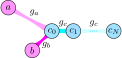
\includegraphics[width=0.8\textwidth, draft=false]{phog/multi_mode}
\end{subfigure}
\caption{\label{fig:coupPhoG} Example coupling matrix $\mathcal{G}$ for the PhoG system.}
\end{figure}
\clearpage
\subsection{Linearized equations}
Letting $n, m \in \left[1, N+2\right], n \ne m$, we derive a closed system of coupled differential equations for first- and second-order expectations

\begingroup
\allowdisplaybreaks
\begin{align}\label{eqn:linearsystem}
% an
\partial_t\langle\hat{a}_n\rangle &= \left(- i \omega_n - \frac{\Gamma_n}{2}\right)\langle\hat{a}_n\rangle - 2 i U \langle\hat{a}_n\rangle\langle\hat{a}_n^\dagger\hat{a}_n\rangle - i U \langle\hat{a}_n^\dagger\rangle\langle\hat{a}_n\hat{a}_n\rangle + 2 i U \langle\hat{a}_n^\dagger\rangle \langle\hat{a}_n\rangle\langle\hat{a}_n\rangle \notag \\
&- \sum_{j=1}^N i \mathcal{G}_{n, j} \langle\hat{a}_j\rangle, \notag \\
%
%
% adn
\partial_t\langle\hat{a}_n^\dagger\rangle &= \left(+ i \omega_n - \frac{\Gamma_n}{2} \right) \langle\hat{a}_n^\dagger\rangle + 2 i U \langle\hat{a}_n^\dagger\rangle\langle\hat{a}_n^\dagger\hat{a}_n\rangle + i U \langle\hat{a}_n\rangle\langle\hat{a}_n^\dagger\hat{a}_n^\dagger\rangle - 2 i U\langle\hat{a}_n^\dagger\rangle\langle\hat{a}_n^\dagger\rangle\langle\hat{a}_n\rangle \notag \\
&+ \sum_{j=1}^N i \mathcal{G}_{n,j}\langle\hat{a}_j^\dagger\rangle, \notag \\
%
%
% anan
\partial_t\langle\hat{a}_n\hat{a}_n\rangle &= \left( - 2 i \omega_n - \Gamma_n\right) \langle\hat{a}_n\hat{a}_n\rangle - 6 i U \langle\hat{a}_n^\dagger \hat{a}_n\rangle \langle\hat{a}_n\hat{a}_n\rangle + 4 i U \langle\hat{a}_n^\dagger\rangle \langle\hat{a}_n\rangle \langle\hat{a}_n\rangle\langle\hat{a}_n\rangle - i U \langle \hat{a}_n\hat{a}_n\rangle \notag \\
&- \sum_{j=1}^N 2 i \mathcal{G}_{n, j}\langle\hat{a}_n\hat{a}_j\rangle,  \notag \\
%
%
% adnan
\partial_t \langle\hat{a}_n^\dagger\hat{a}_n\rangle &= - \Gamma_n\langle\hat{a}_n^\dagger\hat{a}_n\rangle + \Gamma_n \bar{n}_{th}^{\left(n\right)} + \sum_{j=1}^N i \mathcal{G}_{n, j}\left(\langle\hat{a}_j^\dagger\hat{a}_n\rangle - \langle\hat{a}_n^\dagger\hat{a}_j\rangle\right), \notag \\ 
%
%
%
%
% adnadn
\partial_t\langle\hat{a}_n^\dagger\hat{a}_n^\dagger\rangle &= \left(2 i \omega_n - \Gamma_n  \right) \langle\hat{a}_n^\dagger\hat{a}_n^\dagger\rangle + 6 i U \langle\hat{a}_n^\dagger\hat{a}_n^\dagger\rangle\langle\hat{a}_n^\dagger \hat{a}_n\rangle - 4 i U \langle\hat{a}_n^\dagger\rangle\langle\hat{a}_n^\dagger\rangle\langle\hat{a}_n^\dagger\rangle\langle\hat{a}_n\rangle + i U \langle\hat{a}_n\hat{a}^\dagger_n\rangle  \notag \\
&+ \sum_{j=1}^N 2 i \mathcal{G}_{n, j} \langle\hat{a}_n^\dagger\hat{a}_j^\dagger\rangle, \notag \\
%
%
% anam
\partial_t\langle\hat{a}_n\hat{a}_m\rangle &= \left(i\left(\omega_n + \omega_m\right) - \frac{\Gamma_n + \Gamma_m}{2}\right)\langle\hat{a}_n\hat{a}_m\rangle - 2 i U \langle\hat{a}_n^\dagger\hat{a}_n\rangle \langle\hat{a}_n\hat{a}_m\rangle - i U \langle\hat{a}_n^\dagger\hat{a}_m\rangle \langle\hat{a}_n\hat{a}_n\rangle \notag \\
& - 2 i U \langle\hat{a}_m^\dagger\hat{a}_m\rangle\langle\hat{a}_n\hat{a}_m\rangle - i U \langle\hat{a}_m^\dagger\hat{a}_n\rangle\langle\hat{a}_m\hat{a}_m\rangle + 2 i U \langle\hat{a}_n^\dagger\rangle \langle\hat{a}_n\rangle \langle\hat{a}_n\rangle \langle\hat{a}_m\rangle + 2 i U \langle\hat{a}_n\rangle \langle\hat{a}_m^\dagger\rangle \langle\hat{a}_m\rangle\langle\hat{a}_m\rangle \notag \\
& - \sum_{j=1}^N i \mathcal{G}_{n, j}\langle\hat{a}_j\hat{a}_m\rangle - \sum_{q=1}^N i \mathcal{G}_{m, q} \langle\hat{a}_n\hat{a}_q\rangle, \notag \\
%
%
% adnam
\partial_t\langle\hat{a}_n^\dagger\hat{a}_m\rangle &= \left(i\left(\omega_n - \omega_m\right) - \frac{\Gamma_n + \Gamma_m}{2}\right)\langle\hat{a}_n^\dagger\hat{a}_m\rangle + 2 i U \langle\hat{a}_n^\dagger\hat{a}_m \rangle \langle\hat{a}_n^\dagger \hat{a}_n\rangle + i U \langle \hat{a}_n^\dagger \hat{a}_n^\dagger\rangle\langle\hat{a}_n\hat{a}_m\rangle \notag \\
& - 2 i U \langle\hat{a}_n^\dagger \hat{a}_m \rangle \langle \hat{a}_m^\dagger \hat{a}_m\rangle - i U \langle\hat{a}_n^\dagger \hat{a}_m^\dagger\rangle \langle\hat{a}_m\hat{a}_m\rangle - 2 i U \langle\hat{a}_n^\dagger\rangle \langle\hat{a}_n^\dagger\rangle \langle\hat{a}_n\rangle \langle\hat{a}_m\rangle + 2 i U \langle\hat{a}_n^\dagger \rangle \langle \hat{a}_m^\dagger \rangle \langle \hat{a}_m\rangle \langle\hat{a}_m\rangle \notag \\
& + \sum_{j=1}^N i \mathcal{G}_{n, j}\langle\hat{a}_j^\dagger\hat{a}_m\rangle - \sum_{q=1}^N i \mathcal{G}_{m, q}\langle \hat{a}_n^\dagger \hat{a}_q\rangle,  \notag \\
%
%
% adnadm
\partial_t\langle\hat{a}_n^\dagger\hat{a}_m^\dagger\rangle &= \left(i \left(\omega_n + \omega_m\right) - \frac{\Gamma_n + \Gamma_m}{2}\right) \langle \hat{a}_n^\dagger \hat{a}_m^\dagger\rangle + 2 i U \langle\hat{a}_n^\dagger \hat{a}_m^\dagger\rangle \langle \hat{a}_n^\dagger \hat{a}_n\rangle + i U \langle \hat{a}_n^\dagger \hat{a}_n^\dagger \rangle \langle \hat{a}_m^\dagger \hat{a}_n\rangle \notag \\
&+ 2 i U \langle\hat{a}_n^\dagger \hat{a}_m^\dagger \rangle \langle \hat{a}_m^\dagger \hat{a}_m\rangle + i U \langle \hat{a}_n^\dagger \hat{a}_m\rangle \langle \hat{a}_m^\dagger \hat{a}_m^\dagger \rangle - 2 i U \langle\hat{a}_n^\dagger \rangle \langle \hat{a}_n^\dagger \rangle \langle \hat{a}_n \rangle \langle \hat{a}_m^\dagger\rangle - 2 i U \langle \hat{a}_n^\dagger \rangle \langle \hat{a}_m^\dagger \rangle \langle \hat{a}_m^\dagger \rangle \langle \hat{a}_m\rangle \notag \\
& + \sum_{j=1}^N i \mathcal{G}_{n, j} \langle\hat{a}_j^\dagger \hat{a}_m^\dagger\rangle + \sum_{q=1}^N i \mathcal{G}_{m, q} \langle\hat{a}_n^\dagger \hat{a}_q^\dagger\rangle.
\end{align} 
\endgroup

